\documentclass[conference,10pt]{IEEEtran}
\IEEEoverridecommandlockouts
\usepackage[T1]{fontenc}
\usepackage{graphicx,booktabs,amsmath,amssymb,multirow,xcolor,url,xspace}
\usepackage[hidelinks]{hyperref}
\hypersetup{pdftitle={Egocentric Human Demonstrations for Robot Manipulation: Dataset Design, Processing, and an Offline Learnability Analysis}, pdfauthor={Jeong Hwan Lee}}
\usepackage{tikz}
\usetikzlibrary{positioning,arrows.meta,fit,backgrounds}
\newcommand{\mm}{\,mm\xspace}
\newcommand{\cmt}[1]{}

\begin{document}
\title{Egocentric Human Demonstrations for Robot Manipulation:\\Dataset Design, Processing, and an Offline Learnability Analysis}
\author{\IEEEauthorblockN{Jeong Hwan Lee}
\IEEEauthorblockA{Technical report, September 2026 \quad alnrg2arg@gmail.com\\
Code, results and sample data available on request}}
\maketitle

\begin{abstract}
We study how far natural egocentric human demonstrations, recorded with a hand-worn UMI-style gripper, can be turned into
training data for a bimanual robot policy. We collected 349 bimanual demonstrations of a three-cube stacking task with six
stacking orders balanced at collection time (51--64 episodes per order), using per-hand wrist fisheye cameras, IMUs and jaw
encoders plus a fixed head camera. A multi-stage pipeline (MASt3R-SLAM wrist poses with per-episode visual--inertial scale,
retargeting to a 6-DoF robot arm, and synchronisation, workspace, metric and inverse-kinematics gates) keeps 259 episodes, or
561 bimanual 65-frame segments. On these we fine-tune a 0.9B-parameter vision-language-action model (X-VLA) to predict 30-step
joint-space action chunks, and evaluate it offline on 26 held-out episodes. The median held-out TCP error is 1.5--5.7\mm over a
0.2--1.2\,s horizon. This figure is dominated by static phases: on the 23\% of samples in which the target moves at least
20\mm, the error at 1.2\,s is 39.9\mm, direction cosine 0.90, and the policy reduces joint error by 24\% relative to a
zero-motion predictor. Swapping the order instruction changes the predicted motion measurably but by only ${\sim}8\%$ of its
magnitude, and the true instruction predicts the human motion no better than the five wrong ones, so the model makes no
task-useful use of the order instruction in this evaluation.
Two follow-ups address the main bottleneck. Replacing the single-anchor retarget with multi-seed trajectory-window
retrieval raises the usable fraction of candidate segments from 36.5\% to 56.1\% and brings the retargeted postures
much closer to real robot postures; a 60-episode robot-like re-collection is used to test whether collection style changes
retarget feasibility; it does not appreciably, a negative, diagnostic result. Fine-tuned on 150 robot demonstrations, the ego-pretrained model has a
10\% lower geo score than an otherwise identical model trained from scratch (95\% CI 5.6--14.7\%), but only on episodes
contained in both training sets. We report no closed-loop robot results, and no experiment tests new spatial layouts or
unseen stacking orders; we state explicitly which generalization claims this data can and cannot support.
\end{abstract}

\section{Introduction}
Collecting robot demonstrations is often expensive, requiring access to a physical robot, an operator and task-specific
teleoperation infrastructure. Egocentric human
demonstrations can be collected faster, with less hardware, in natural settings, and hand-worn grippers such as UMI~\cite{chi2024umi}
make the human's end-effector look like the robot's, reducing the embodiment gap at the gripper. Whether such data
transfers to a specific robot depends on a chain of steps that is rarely audited end to end: sensor calibration, metric pose
recovery from a moving wrist camera, retargeting into the robot's kinematics, and the filtering that decides which human motion
is kept at all. Each step can silently change what a policy ends up learning.

This report documents one complete pass through that chain on real data and asks a deliberately narrow question:
\emph{after all processing, how much robot-executable action structure does a pretrained vision-language-action (VLA) model
learn from retargeted egocentric human demonstrations, and does it use the task-order instruction?} Our contributions are:
\begin{itemize}
\item a 349-episode bimanual egocentric dataset of three-cube stacking with six balanced stacking orders, with full sensor
calibration and per-episode metadata (Sec.~\ref{sec:data});
\item a documented processing funnel from raw human video to robot joint-space segments, reporting what each gate removes
(Sec.~\ref{sec:proc});
\item an offline evaluation of a 0.9B-parameter VLA fine-tuned on the result, including a motion-gated analysis showing that
aggregate errors are dominated by static phases, and a prompt-swap test of instruction use (Secs.~\ref{sec:eval}--\ref{sec:fail});
\item follow-up experiments on the retargeting bottleneck, robot-like re-collection and ego-to-robot fine-tuning (Sec.~\ref{sec:follow}).
\end{itemize}
We are explicit about scope. The evaluation is open-loop on held-out \emph{episodes}; it is not a closed-loop robot test,
and because layouts were not recorded and all six orders appear in training, it measures neither spatial nor task-order
generalization. Sec.~\ref{sec:lim} lists the experiments needed for those claims.

\section{Related and Motivating Work}
\textbf{Portable demonstration interfaces.} UMI~\cite{chi2024umi} records hand-held gripper demonstrations with a wrist fisheye
camera and recovers poses with ORB-SLAM3 against a per-scene map; DexCap~\cite{wang2024dexcap} and related systems target dexterous
hands. Our device follows UMI's wrist-camera design but adds an IMU and a jaw encoder per hand and a fixed head camera.
\textbf{Learning from egocentric humans.} EgoMimic~\cite{kareer2024egomimic} and MimicPlay~\cite{wang2023mimicplay} co-train robot
policies on human egocentric video and robot data; large egocentric corpora such as Ego4D~\cite{grauman2022ego4d} motivate the
scaling argument. These works report closed-loop gains; we instead audit what survives processing and what a model learns
offline, which is a prerequisite for interpreting such gains.
\textbf{Policies.} Action-chunking imitation (ACT~\cite{zhao2023act}, Diffusion Policy~\cite{chi2023diffusion}) and VLA models
(OpenVLA~\cite{kim2024openvla}, $\pi_0$~\cite{black2024pi0}, X-VLA~\cite{zheng2025xvla}) predict multi-step action chunks from
images and language. We use X-VLA through LeRobot~\cite{cadene2024lerobot} because its flow-matching~\cite{lipman2023flow} head
and soft prompts accommodate a new embodiment with a small dataset.
\textbf{Pose recovery.} MASt3R-SLAM~\cite{murai2025mast3rslam} provides dense monocular SLAM from a 3D reconstruction prior; we
combine it with IMU-based scale estimation, calibrated with Kalibr~\cite{furgale2013kalibr}.

\begin{figure*}[t]
\centering
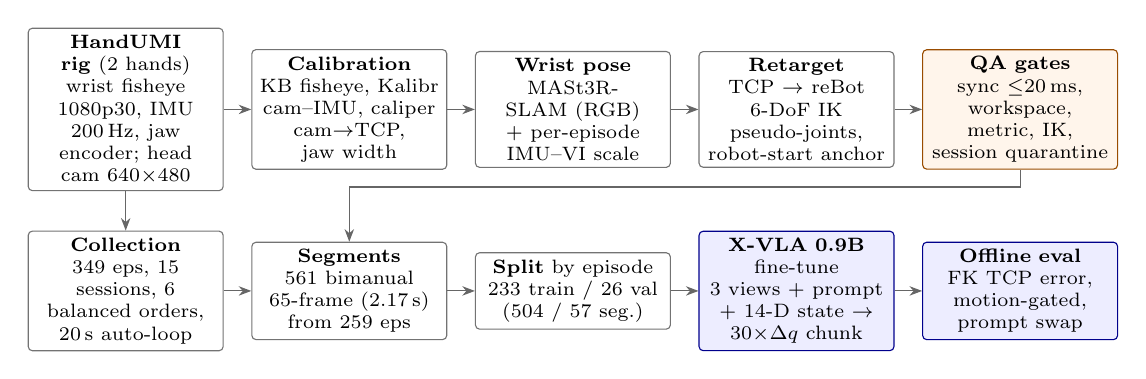
\begin{tikzpicture}[font=\scriptsize, node distance=3.5mm and 3.5mm,
  box/.style={draw=black!55, rounded corners=1.5pt, align=center, inner sep=2.5pt, minimum height=9.5mm, text width=23mm, fill=white},
  gate/.style={box, fill=orange!8, draw=orange!60!black},
  learn/.style={box, fill=blue!7, draw=blue!55!black},
  arr/.style={-{Stealth[length=1.6mm]}, draw=black!60}]
\node[box] (dev) {\textbf{HandUMI rig} (2 hands)\\wrist fisheye 1080p30, IMU 200\,Hz, jaw encoder; head cam 640$\times$480};
\node[box, right=of dev] (cal) {\textbf{Calibration}\\KB fisheye, Kalibr cam--IMU, caliper cam$\to$TCP, jaw width};
\node[box, right=of cal] (pose) {\textbf{Wrist pose}\\MASt3R-SLAM (RGB) + per-episode IMU--VI scale};
\node[box, right=of pose] (ret) {\textbf{Retarget}\\TCP $\to$ reBot 6-DoF IK pseudo-joints, robot-start anchor};
\node[gate, right=of ret] (qa) {\textbf{QA gates}\\sync $\le$20\,ms, workspace, metric, IK, session quarantine};
\node[box, below=5mm of dev] (col) {\textbf{Collection}\\349 eps, 15 sessions, 6 balanced orders, 20\,s auto-loop};
\node[box, right=of col] (seg) {\textbf{Segments}\\561 bimanual 65-frame (2.17\,s) from 259 eps};
\node[box, right=of seg] (split) {\textbf{Split} by episode\\233 train / 26 val (504 / 57 seg.)};
\node[learn, right=of split] (vla) {\textbf{X-VLA 0.9B} fine-tune\\3 views + prompt + 14-D state $\to$ 30$\times$$\Delta q$ chunk};
\node[learn, right=of vla] (ev) {\textbf{Offline eval}\\FK TCP error, motion-gated, prompt swap};
\draw[arr] (dev)--(cal); \draw[arr] (cal)--(pose); \draw[arr] (pose)--(ret); \draw[arr] (ret)--(qa);
\draw[arr] (dev)--(col); \draw[arr] (qa.south) |- ++(0,-2.2mm) -| (seg.north);
\draw[arr] (col)--(seg); \draw[arr] (seg)--(split); \draw[arr] (split)--(vla); \draw[arr] (vla)--(ev);
\end{tikzpicture}
\caption{System and data pipeline. Orange: filtering stages whose losses are reported in Table~\ref{tab:funnel}; blue: learning
and evaluation. No stage uses robot rollouts.}
\label{fig:pipeline}
\end{figure*}

\section{Dataset and Task Design}\label{sec:data}
\textbf{Hardware.} Each hand wears a HandUMI unit: a 1920$\times$1080, 30\,fps fisheye camera, a 200\,Hz IMU and a jaw encoder
sampled at 100\,Hz. A fixed head-mounted Logitech C922 records a 640$\times$480, 30\,fps view of the table; this is the global
view given to the policy (Fig.~\ref{fig:dataset}a). All streams are written to one MCAP file and three videos per episode.

\textbf{Task.} Three 50\mm cubes (red, blue, purple) are stacked on a fixed plate in one of six orders; the instruction names the
order, e.g.\ ``Stack the blue cube on the bottom, purple cube in the middle, and red cube on the top, on the plate.'' An
auto-loop records a 20\,s take after spoken cues and gives a 10\,s reset in which the operator re-places the cubes by hand.
The next order is the least-collected one (target 50 per order), so orders are \emph{balanced}, not randomized. The cube
layout varies between episodes through the manual reset, around a nominal layout matched to our robot workspace, but it
was not recorded; there is no per-episode layout label.

\textbf{Collection.} One operator recorded 349 episodes in 15 sessions over three days (15--17 September 2026), 2.20\,h in
total (median episode 23.05\,s). Per order: RBP 64, RPB 62, BRP 61, BPR 56, PRB 55, PBR 51 (Fig.~\ref{fig:dataset}b). Episodes from ten early sessions (55 episodes) are tracked as a separate provenance domain (``early'') from the main 294, because
their gripper anchors were derived afterwards; after filtering the two domains behave alike.

\textbf{Calibration.} Wrist cameras use a Kannala--Brandt fisheye model (left $f_x{=}789$, right $f_x{=}791$\,px). Kalibr
camera--IMU calibration gives time offsets of 30.2 and 32.8\,ms with mean reprojection errors of 6.0 and 5.6\,px, which is
high and one reason pose accuracy is validated separately (Sec.~\ref{sec:proc}). The camera-to-TCP transform is a caliper
measurement, $t=[0, 55.3, 122.5]$\mm with a fixed axis permutation, following UMI's use of a CAD constant; it was measured on
one unit and applied to both. The jaw-width scale (aperture $67.5\pm5$\mm) is estimated from video of 50\mm-cube grasps; a
caliper check is pending.

\begin{figure*}[t]
\centering
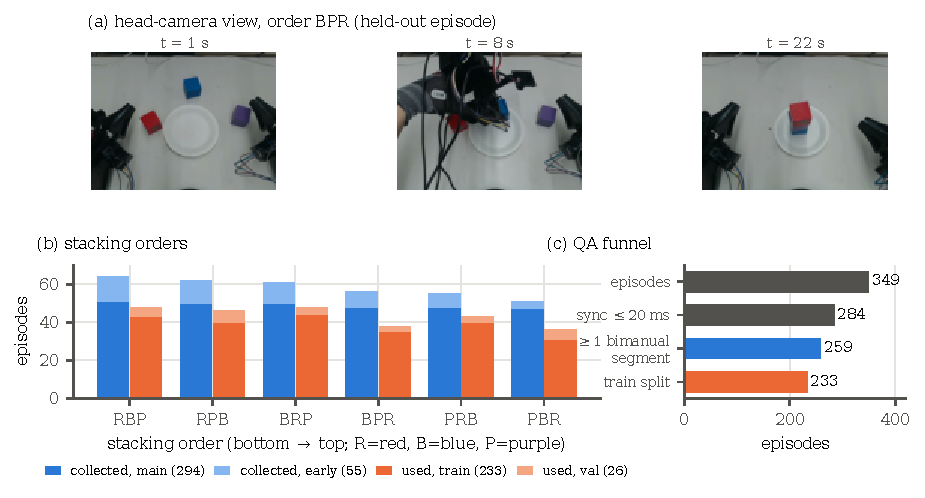
\includegraphics[width=\textwidth]{figures/fig2_dataset.pdf}
\caption{Dataset design. (a) Head-camera frames at 1, 8 and 22\,s of a held-out episode (order BPR). (b) Episodes per stacking order, as collected
(main/early domains) and after processing (train/val). (c) Episode-level QA funnel.}
\label{fig:dataset}
\end{figure*}

\section{Processing and Splits}\label{sec:proc}
\textbf{Wrist poses.} UMI localizes all demonstrations in one ORB-SLAM3 map per scene. On our data this failed: maps built
before a scene change did not relocalize, and on a marker benchmark (below) its tracks cover a median of 3\% of each demonstration, with frequent position
reversals (median reversal rate 0.24 versus 0.07 for the method we adopt). We therefore run MASt3R-SLAM on the RGB wrist video alone and recover metric scale
per episode from the IMU (visual--inertial fit over a 15-frame window). On a separate benchmark of 14 ArUco-marker episodes
(28 hand trajectories; 10 held out), run on the same GPU as the dataset, this gives median tracking coverage 1.00 versus 0.03
for ORB-SLAM3 with a stored map, scale error p50/p90 of 4.6/17.0\% (versus 18.5/23.8\% for one global constant), rotation error p50/p90 0.84/2.13\textdegree{} and a UMI-style 16-step relative
position error p90 of 11.3\mm. The 349 episodes themselves have no ground truth.

\textbf{Retargeting.} Each TCP trajectory is mapped to a reBot B601 6-DoF arm by inverse kinematics on its URDF. Absolute
workspace geometry is not recoverable across episodes, so each segment is re-anchored at a fixed robot start pose (the median
active pose of our robot teleoperation data); motion is transferred, absolute cube positions are not. The jaw encoder becomes a
binary gripper command.

\textbf{Gates.} Table~\ref{tab:funnel} lists the funnel. 65 episodes fail the $\le$20\,ms synchronisation requirement for a full
65-frame window; the remaining 284 yield 1{,}306 candidate bimanual segments, of which 677 leave the robot workspace, 50 fail the
metric-scale check and 18 fail IK, leaving 561 (43.0\%). Two sessions (6 episodes) were quarantined for an IMU--camera
rotation inconsistency; none contributed a segment. The training unit is a 65-frame (2.17\,s) segment; 47\% of segments start
in the first 5\,s of an episode.

\textbf{Split.} The 259 episodes with at least one bimanual segment are split at random by episode (seed 0, 10\%): 233 train /
26 val, i.e.\ 504/57 segments and 32{,}760/3{,}705 frames. No episode spans both sides. The split is not stratified; validation
has 3--6 episodes per order, 22 main / 4 early, from 9 of the 13 non-quarantined sessions.

\begin{table}[t]
\centering\footnotesize
\caption{Processing funnel (counts recomputed from the census files in the repository).}
\label{tab:funnel}
\setlength{\tabcolsep}{4pt}\begin{tabular}{@{}lrr@{}}
\toprule
Stage & Episodes & Segments \\
\midrule
Recorded (KEEP) & 349 & -- \\
Pose + gripper exported (698 tracks) & 349 & -- \\
Sync $\le$20\,ms, $\ge$65-frame window & 284 & 1{,}306 \\
\quad $-$ workspace / metric scale / IK & & $-$677 / $-$50 / $-$18 \\
$\ge$1 bimanual segment (training pool) & 259 & 561 \\
\quad train / val (by episode, seed 0) & 233 / 26 & 504 / 57 \\
\bottomrule
\end{tabular}
\end{table}

\section{Model and Training}\label{sec:model}
We fine-tune X-VLA~\cite{zheng2025xvla} (LeRobot implementation) from the public \texttt{xvla-base} checkpoint: a Florence-2
vision-language encoder~\cite{xiao2024florence2} and a 24-layer transformer policy (hidden 1024, 16 heads, 32 soft prompts) with a
flow-matching action head (10 denoising steps); 879M parameters, all trainable. Inputs are the three views (head, left wrist,
right wrist; resized to 224\,px), the order instruction and a 14-D state (6 joint angles and a binary gripper per arm).

\textbf{Action target.} For state time $t$ the model predicts a 30-step chunk $a_i = q_{t+5+i}-q_t$, $i=0,\dots,29$, of
cumulative joint displacements of the retargeted pseudo-joints (a 5-frame lead, so the chunk covers 0.2--1.17\,s ahead), plus
the absolute gripper command. Two auxiliary terms tie joint space to the measured human motion: (C) the relative TCP position
of the measured trajectory, predicted in spare action dimensions (weight 2.0), and (D) a forward-kinematics loss between
$\mathrm{FK}(q_t+\hat a_i)$ and the measured TCP position (weight 20). Targets are the measured human transitions, never
relabelled robot commands.

\textbf{Optimization.} 300k steps, batch 4, AdamW (lr $10^{-4}$, weight decay $10^{-4}$, 1k warm-up, cosine decay to
$2.5\times10^{-6}$), gradient clipping 10, fp32, one RTX~4090. A checkpoint is saved every 10k steps.
The checkpoint selection rule, minimum geo score (below) on all validation samples, was fixed before training.

\section{Evaluation Protocol}\label{sec:eval}
Evaluation is open-loop on the 26 held-out episodes: from each of the 57 validation segments we take 7 start frames (every 5
frames in 0--30), giving 399 samples and 798 arm-samples, and compare the predicted chunk against the recorded future.
For horizons $k\in\{1,4,8,16,30\}$ we report the TCP position error between $\mathrm{FK}(q_t+\hat a_k)$ and the measured TCP
(median, mm), the joint MAE and that of a \emph{zero-motion} predictor ($\hat a\equiv0$), and the cosine between predicted and
measured TCP displacement. The \emph{geo score} is the mean of the median TCP error over the five horizons. Because most samples
are near-static, we also report every metric on the \emph{moving} subset, arm-samples whose measured TCP moves $\ge$20\mm by $k{=}30$
(187 of 798, 23.4\%). This gate was added after the 60k checkpoint had been evaluated and is used for reporting only.

\textbf{Prompt swap.} To test instruction use, we query the final checkpoint on every sample with each of the six order
instructions using the same noise seed, and with the true instruction under two further seeds. The spread of the six
predictions measures the instruction's effect; the spread across seeds is the sampling-noise floor.

\textbf{What the split does not test.} Validation episodes share operator, scene, sessions and all six orders with training,
and layouts are unlabelled. The results therefore measure within-distribution generalization to new \emph{episodes}, not to new
layouts, orders or scenes.

\section{Results}\label{sec:results}
\begin{table*}[t]
\centering\footnotesize
\setlength{\tabcolsep}{7pt}
\caption{Offline held-out results (26 episodes). TCP error: median FK position error (mm); MAE: joint MAE (deg), with the
zero-motion predictor in parentheses; cos: TCP direction cosine. 160k is the pre-registered selection, 300k the final step.}
\label{tab:results}
\begin{tabular}{@{}llccccc@{}}
\toprule
 & & \multicolumn{5}{c}{horizon $k$ (steps of 1/30\,s after a 5-frame lead)} \\
\cmidrule(l){3-7}
Subset & Metric & 1 & 4 & 8 & 16 & 30 \\
\midrule
\multirow{3}{*}{All (798)} & TCP err., 160k & 1.3 & 1.7 & 2.2 & 3.1 & 5.7 \\
 & TCP err., 300k & 1.5 & 1.8 & 2.2 & 3.2 & 5.7 \\
 & MAE, 300k & 0.30 (0.15) & 0.34 (0.19) & 0.42 (0.25) & 0.57 (0.36) & 0.97 (0.51) \\
\midrule
\multirow{4}{*}{Moving (187)} & TCP err., 160k & 11.2 & 15.0 & 19.9 & 29.2 & 39.1 \\
 & TCP err., 300k & 11.2 & 15.0 & 19.4 & 29.3 & 39.9 \\
 & MAE, 300k & 2.02 (2.32) & 2.68 (3.36) & 3.29 (4.38) & 4.30 (6.34) & 6.59 (8.68) \\
 & cos, 300k & 0.72 & 0.80 & 0.84 & 0.86 & 0.90 \\
\bottomrule
\end{tabular}
\end{table*}

Table~\ref{tab:results} and Fig.~\ref{fig:eval} summarize the evaluation. Four findings stand out.

\textbf{(1) Aggregate errors mostly reflect static phases.} The geo score reaches 2.78\mm at 160k and 2.88\mm at 300k and is
flat after about 120k (Fig.~\ref{fig:eval}a). On moving samples, however, the error is an order of magnitude larger: 11\mm at the
shortest horizon and 40\mm at $k{=}30$, with a p90 of 90\mm; the moving-subset geo score is 23.0\mm versus 2.9\mm on all
samples.

\textbf{(2) On moving samples the policy predicts the direction of motion and beats a no-motion baseline.} The direction
cosine rises from 0.72 at $k{=}1$ to 0.90 at $k{=}30$, and joint MAE is 13--32\% lower than the zero-motion predictor across
horizons (6.59 versus 8.68\textdegree{} at $k{=}30$; Fig.~\ref{fig:eval}b). The model captures the direction of the upcoming motion, not only its presence.

\textbf{(3) On all samples, the policy is worse than predicting no motion.} Joint MAE is about twice the zero-motion MAE at
every horizon (0.30 versus 0.15\textdegree{} at $k{=}1$): during static phases the policy predicts small spurious motion, and the
median predicted-to-measured displacement ratio is 1.41 at $k{=}1$. At $k{=}30$ the spread of predictions is 0.77 of the spread
of targets, so the long horizon is somewhat under-dispersed rather than collapsed.

\textbf{(4) The order instruction changes predictions but does not improve them.} In the prompt swap
(Fig.~\ref{fig:eval}c), the six instructions move the predicted TCP by a median of 4.8\mm at $k{=}30$ on moving samples, about
50$\times$ the sampling-noise spread (0.09\mm) but only 8\% of the predicted displacement (62\mm). The true instruction is not
closer to the recorded motion than the wrong ones: its error is 39.9\mm versus 39.5\mm for the mean wrong instruction, and its
mean rank among the six is 3.55 (chance 3.5; rank 1 in 16\% of cases, chance 17\%), with the same picture at every horizon and
on all samples. The prediction with the true instruction and the original seed reproduces the reference evaluation to within
$10^{-5}$\mm. A caveat is that much of a 2.2\,s segment is order-independent (reaching, lifting); a test restricted to
choice points (the first reach of an episode) needs more such samples than the 26 validation episodes provide.

Per-order breakdowns are in the repository; with 3--6 validation episodes per order they are too small to rank orders, and we do
not interpret differences between them.

\begin{figure*}[t]
\centering
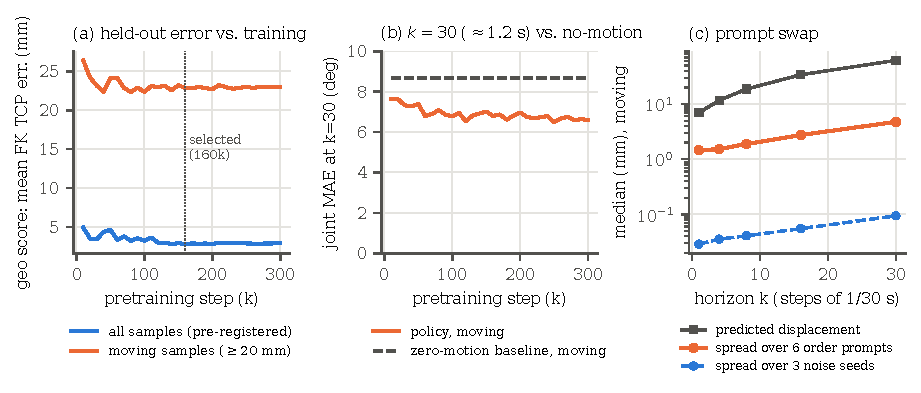
\includegraphics[width=\textwidth]{figures/fig4_eval.pdf}
\caption{Offline evaluation. (a) Geo score over training on all versus moving held-out samples; the pre-registered rule
selects 160k. (b) Joint MAE at $k{=}30$ on moving samples, policy versus zero-motion predictor. (c) Prompt swap on the final
checkpoint: prediction spread across the six order instructions (same seed) versus across three noise seeds (true instruction).}
\label{fig:eval}
\end{figure*}

\section{Failure Analysis}\label{sec:fail}
\textbf{Weak use of the task-order instruction.} The order prompt measurably changes the prediction, but this variation does
not improve agreement with the recorded motion (finding 4).
In this dataset the order is also partly visible from the scene once stacking has begun, so the instruction is only necessary
at the start of an episode; nothing in training forces the model to use it.

\textbf{Static-phase drift.} The dominant error mode is non-zero motion predicted while the human is still. It is the reason
the all-samples MAE exceeds the zero-motion baseline, and on a robot it would appear as creep before grasps or after placement.
One plausible contributor, not yet tested, is residual pose noise in near-static windows, which makes ``stationary'' targets noisy.

\textbf{Long-horizon under-dispersion.} Predictions at $k{=}30$ vary less than the targets (ratio 0.77) and the p90 error on
moving samples reaches 90\mm, so fast or unusual motions are pulled towards the mean.

\textbf{Data lost before learning.} 57\% of the candidate segments are removed; the workspace gate accounts for 677 of the 745
removals (91\%), and in 531 of those (78\%) only one arm leaves the robot workspace. Because the gate removes motions by
their extent, the kept set is likely biased towards compact motions; we have not yet quantified this bias.

\textbf{Upstream failures that shaped the design.} ORB-SLAM3 with a stored map failed to relocalize across scene changes and
produced position jitter; a camera-orientation convention error in an earlier export corrupted rotations until it was found by a frame-regression test; and 65 episodes (19\%) fail synchronisation. Each was found by an explicit gate,
not by training loss.

\section{Follow-up Experiments}\label{sec:follow}
\textbf{Retargeting v2.} The single start anchor of Sec.~\ref{sec:proc} was the main source of loss: every segment began at
one robot posture, so most left the workspace and the retargeted joint trajectories covered one posture cluster. We replaced
it with multi-seed retargeting under a strict budget: every real-robot quantity (seed bank, workspace gate, posture
penalty, trajectory windows) comes from 30 robot episodes only, and results are measured against a disjoint set of 120
robot episodes. Table~\ref{tab:retarget} compares four variants on the same 1{,}229 candidate segments. Trajectory-window
retrieval (TR), which starts each human segment from the closest feasible robot trajectory window, is the most
robot-like: posture distance to the held-out robot data falls from 1.49 to 0.27\,rad (median) and start postures span 100
clusters instead of 1. It solves fewer segments than the kinematic variants because it cannot place fast motions; among the
686 segments both TR and the penalised kinematic variant solve, their joint-velocity distributions are similar (W1 0.00207
vs 0.00226), so the posture gain, not a dynamics gain, is what TR adds. The remaining failures are almost all ``no
workspace-compatible window'' (399 of 402 unsolved).

\begin{table}[t]
\centering\footnotesize\setlength{\tabcolsep}{3.5pt}
\caption{Retargeting variants on the 1{,}229 candidate segments of the 259 episodes, measured against 120 held-out robot
episodes. NN: nearest-neighbour joint-space distance to robot postures (rad, p50/p90); W1: Wasserstein distance of
$|\Delta q|$ per step.}
\label{tab:retarget}
\begin{tabular}{@{}lcccc@{}}
\toprule
Variant & Usable & NN p50 / p90 & Start clusters & W1 $|\Delta q|$ \\
\midrule
v1 single anchor & 36.5\% & 1.49 / 1.55 & 1 & 0.00197 \\
v2-K multi-seed IK & 66.6\% & 1.21 / 1.60 & -- & 0.00275 \\
v2-Kr + posture penalty & 67.0\% & 0.44 / 0.74 & -- & 0.00310 \\
v2-TR window retrieval & 56.1\% & 0.27 / 0.45 & 100 & 0.00208 \\
\bottomrule
\end{tabular}
\end{table}

\textbf{Robot-like re-collection.} To test whether the loss is a collection-style problem, we added a robot-like protocol to
the collector (30\,s takes, live wrist-rotation speed and grasp feedback against robot statistics) and recorded 60 new
episodes (10 per order) in one session. Its interpretation rules were fixed before retargeting. Live rotation speed halved
(median over-threshold fraction 0.144 to 0.067), but the per-episode TR yield did not change (0.59 vs 0.59) and TR usable
rose only from 56.1\% to 58.9\%; the per-episode correlation between live robot-likeness and TR yield is weak
(Spearman $\rho=-0.11$, $p=0.05$, pooled $n=316$). Robot-like movement, as measured live, is associated with, but not a
proxy for, retarget feasibility; workspace placement remains the main failure. The final TR dataset combines both
collections: 996 segments (896 train / 100 val) from 316 source episodes, with the original 689 segments preserved
bit-identically.

\textbf{Ego pretraining for robot fine-tuning.} The first-release ego checkpoint (Sec.~\ref{sec:model}) and the base
checkpoint were each fine-tuned on 150 robot teleoperation episodes of the same task with the same recipe, data and
evaluation; only the initialization differs. At the matched step of 250k, the ego-initialized model has a 10.0\% lower geo
score (episode-level paired bootstrap, 10k draws: 95\% CI $-14.7$ to $-5.6\%$), a 7.2\% lower moving-sample geo score (CI
$-13.4$ to $-1.8\%$) and 6.8\% lower moving joint MAE at $k{=}30$ (CI $-12.7$ to $+0.5\%$); 8 of the 10 evaluation
episodes favour it. The evaluation episodes are part of both fine-tuning sets, so this measures how well each model fits
the robot training distribution, not generalization. A smaller-data comparison on 90 robot episodes was stopped early with
only two matched steps (10k, 20k); there the signs are mixed (all-sample geo $-33\%$ and $-11\%$, moving-sample geo $+2\%$ and
$+13\%$ for the ego initialization), so we draw no conclusion from it.

\textbf{Pretraining on the final dataset.} X-VLA was pretrained from \texttt{xvla-base} on the 996-segment dataset with
the same recipe (planned 300k steps). The run was stopped at 211.7k steps; the 100k and 200k checkpoints are kept, with 100k
designated as the initialization for later robot fine-tuning. No robot fine-tuning result from these checkpoints is
reported here: the only fine-tuning comparison above uses the first-release ego checkpoint.

\section{Limitations and Future Work}\label{sec:lim}
\textbf{Completed:} dataset collection and calibration; the pose, retargeting and QA pipeline; 300k-step ego fine-tuning and
offline evaluation on held-out episodes; retargeting v2, the robot-like re-collection and the matched 150-episode robot
fine-tuning comparison; pretraining on the final 996-segment dataset (stopped at 211.7k steps, checkpoints 100k and 200k).
\textbf{Stopped early, no conclusion:} the 90-, 60- and 30-episode robot fine-tuning comparisons (at most two matched steps,
or only one arm run). \textbf{Not yet done:} robot fine-tuning from the final-dataset checkpoints. The robot evaluation
episodes overlap the fine-tuning data, so a benefit on disjoint robot data remains to be shown.

\textbf{Not supported by this study:} (i) closed-loop success on a robot; (ii) generalization to new cube layouts, since layouts
were not recorded and absolute geometry is discarded by design; (iii) generalization to unseen stacking orders, since all six
orders appear in training; (iv) transfer beyond one operator, one scene and three days; (v) any benefit of human data for robot learning beyond fitting the robot training distribution. \textbf{Planned experiments:} record layouts from the head camera and hold out layout regions; hold out two orders
entirely and test instruction following; train with a static-phase-aware loss or weighting; evaluate closed-loop on the robot
with the order instruction as the controlled variable.

More broadly, this work is a first step towards a research agenda in which egocentric human demonstrations provide scalable
supervision for robot policies: learning human-to-robot representations that keep task geometry and intent while discarding
embodiment detail, and evaluating them with predictive world models before execution. The present results show that the
bottleneck is as much in pose recovery, filtering and evaluation design as in the policy.

\section{Conclusion}
We collected 349 bimanual egocentric demonstrations of three-cube stacking, processed them into 561 robot joint-space segments
through a gated pipeline, and fine-tuned a 0.9B VLA on the result. Offline, on moving samples the model predicts the
direction of held-out human motion reliably (cosine 0.90 at $k{=}30$) and reduces joint-space error relative to a zero-motion
baseline (by 13--32\% across horizons); on static samples it predicts spurious motion, aggregate metrics hide this, and
swapping the order instruction does not make predictions more accurate. Multi-seed trajectory retrieval removes much of the retargeting loss, and ego pretraining gives a small, consistent gain
when fine-tuning on robot data, measured on the robot training episodes. Spatial and task-order generalization, a benefit on
disjoint robot data, and closed-loop transfer remain open and require the controlled experiments listed above.

\begin{thebibliography}{99}\footnotesize
\bibitem{chi2024umi} C.~Chi, Z.~Xu, C.~Pan, E.~Cousineau, B.~Burchfiel, S.~Feng, R.~Tedrake, and S.~Song, ``Universal manipulation interface: In-the-wild robot teaching without in-the-wild robots,'' in \emph{RSS}, 2024.
\bibitem{wang2024dexcap} C.~Wang, H.~Shi, W.~Wang, R.~Zhang, L.~Fei-Fei, and C.~K. Liu, ``DexCap: Scalable and portable mocap data collection system for dexterous manipulation,'' in \emph{RSS}, 2024.
\bibitem{kareer2024egomimic} S.~Kareer \emph{et al.}, ``EgoMimic: Scaling imitation learning via egocentric video,'' \emph{arXiv:2410.24221}, 2024.
\bibitem{wang2023mimicplay} C.~Wang \emph{et al.}, ``MimicPlay: Long-horizon imitation learning by watching human play,'' in \emph{CoRL}, 2023.
\bibitem{grauman2022ego4d} K.~Grauman \emph{et al.}, ``Ego4D: Around the world in 3,000 hours of egocentric video,'' in \emph{CVPR}, 2022.
\bibitem{zhao2023act} T.~Z. Zhao, V.~Kumar, S.~Levine, and C.~Finn, ``Learning fine-grained bimanual manipulation with low-cost hardware,'' in \emph{RSS}, 2023.
\bibitem{chi2023diffusion} C.~Chi, S.~Feng, Y.~Du, Z.~Xu, E.~Cousineau, B.~Burchfiel, and S.~Song, ``Diffusion policy: Visuomotor policy learning via action diffusion,'' in \emph{RSS}, 2023.
\bibitem{kim2024openvla} M.~J. Kim \emph{et al.}, ``OpenVLA: An open-source vision-language-action model,'' in \emph{CoRL}, 2024.
\bibitem{black2024pi0} K.~Black \emph{et al.}, ``$\pi_0$: A vision-language-action flow model for general robot control,'' \emph{arXiv:2410.24164}, 2024.
\bibitem{zheng2025xvla} J.~Zheng \emph{et al.}, ``X-VLA: Soft-prompted transformer as scalable cross-embodiment vision-language-action model,'' in \emph{ICLR}, 2026 (arXiv:2510.10274).
\bibitem{cadene2024lerobot} R.~Cadene \emph{et al.}, ``LeRobot: State-of-the-art machine learning for real-world robotics in PyTorch,'' \url{https://github.com/huggingface/lerobot}, 2024.
\bibitem{lipman2023flow} Y.~Lipman, R.~T.~Q. Chen, H.~Ben-Hamu, M.~Nickel, and M.~Le, ``Flow matching for generative modeling,'' in \emph{ICLR}, 2023.
\bibitem{murai2025mast3rslam} R.~Murai, E.~Dexheimer, and A.~J. Davison, ``MASt3R-SLAM: Real-time dense SLAM with 3D reconstruction priors,'' in \emph{CVPR}, 2025.
\bibitem{furgale2013kalibr} P.~Furgale, J.~Rehder, and R.~Siegwart, ``Unified temporal and spatial calibration for multi-sensor systems,'' in \emph{IROS}, 2013.
\bibitem{xiao2024florence2} B.~Xiao \emph{et al.}, ``Florence-2: Advancing a unified representation for a variety of vision tasks,'' in \emph{CVPR}, 2024.
\end{thebibliography}
\end{document}
